
\subsection{Setting 2: Function Selection}

In this section, we study the ability of our method to recover 
the support of the true function.
We use RBF kernels on each group by setting kernel bandwidths
for each dimension as same as above.
Extending the generative model in \cite{ravikumar09spam}, 
we generate observations from the following
50-dimensional additive model:
\begin{align*}
	y_i =& f_1(x_{i1}) + f_2(x_{i2}) + f_3(x_{i3}) + f_4(x_{i4}) + \\
&f_1(x_{i5}x_{i6}) + f_2(x_{i7}x_{i8}) + \\
&f_3(x_{i9}x_{i10}) + f_4(x_{i11}x_{i12}) + \epsilon_i \\
f_1(x) =& -2\sin(2x), f_2(x) = x^2 - \frac{1}{3}, \\
f_3(x)=& x-\frac{1}{2}, f_4(x) = e^{-x} + e^{-1} - 1
\end{align*}
with noise $\epsilon_i \sim \mathcal{N}(0,1)$.
Thus, 46 out of 50 individual features are irrelevant, and
1221 out of 1225 pairwise features are irrelevant.

We then run our method where the component kernels
defined over all single dimensions and pairs of dimensions.
We plot the solution path for two independent datasets, 
with $n=200$ and $n=600$ observations, respectively.
Our results are shown in Figure \ref{fig:n200}.
With $n=600$ samples, at $\lambda=200$ we recover all true nonzero functions for a true positive rate of $100\%$ and have 47 false negatives for a false positive rate of $3.7\%$.

\begin{figure}
\centering
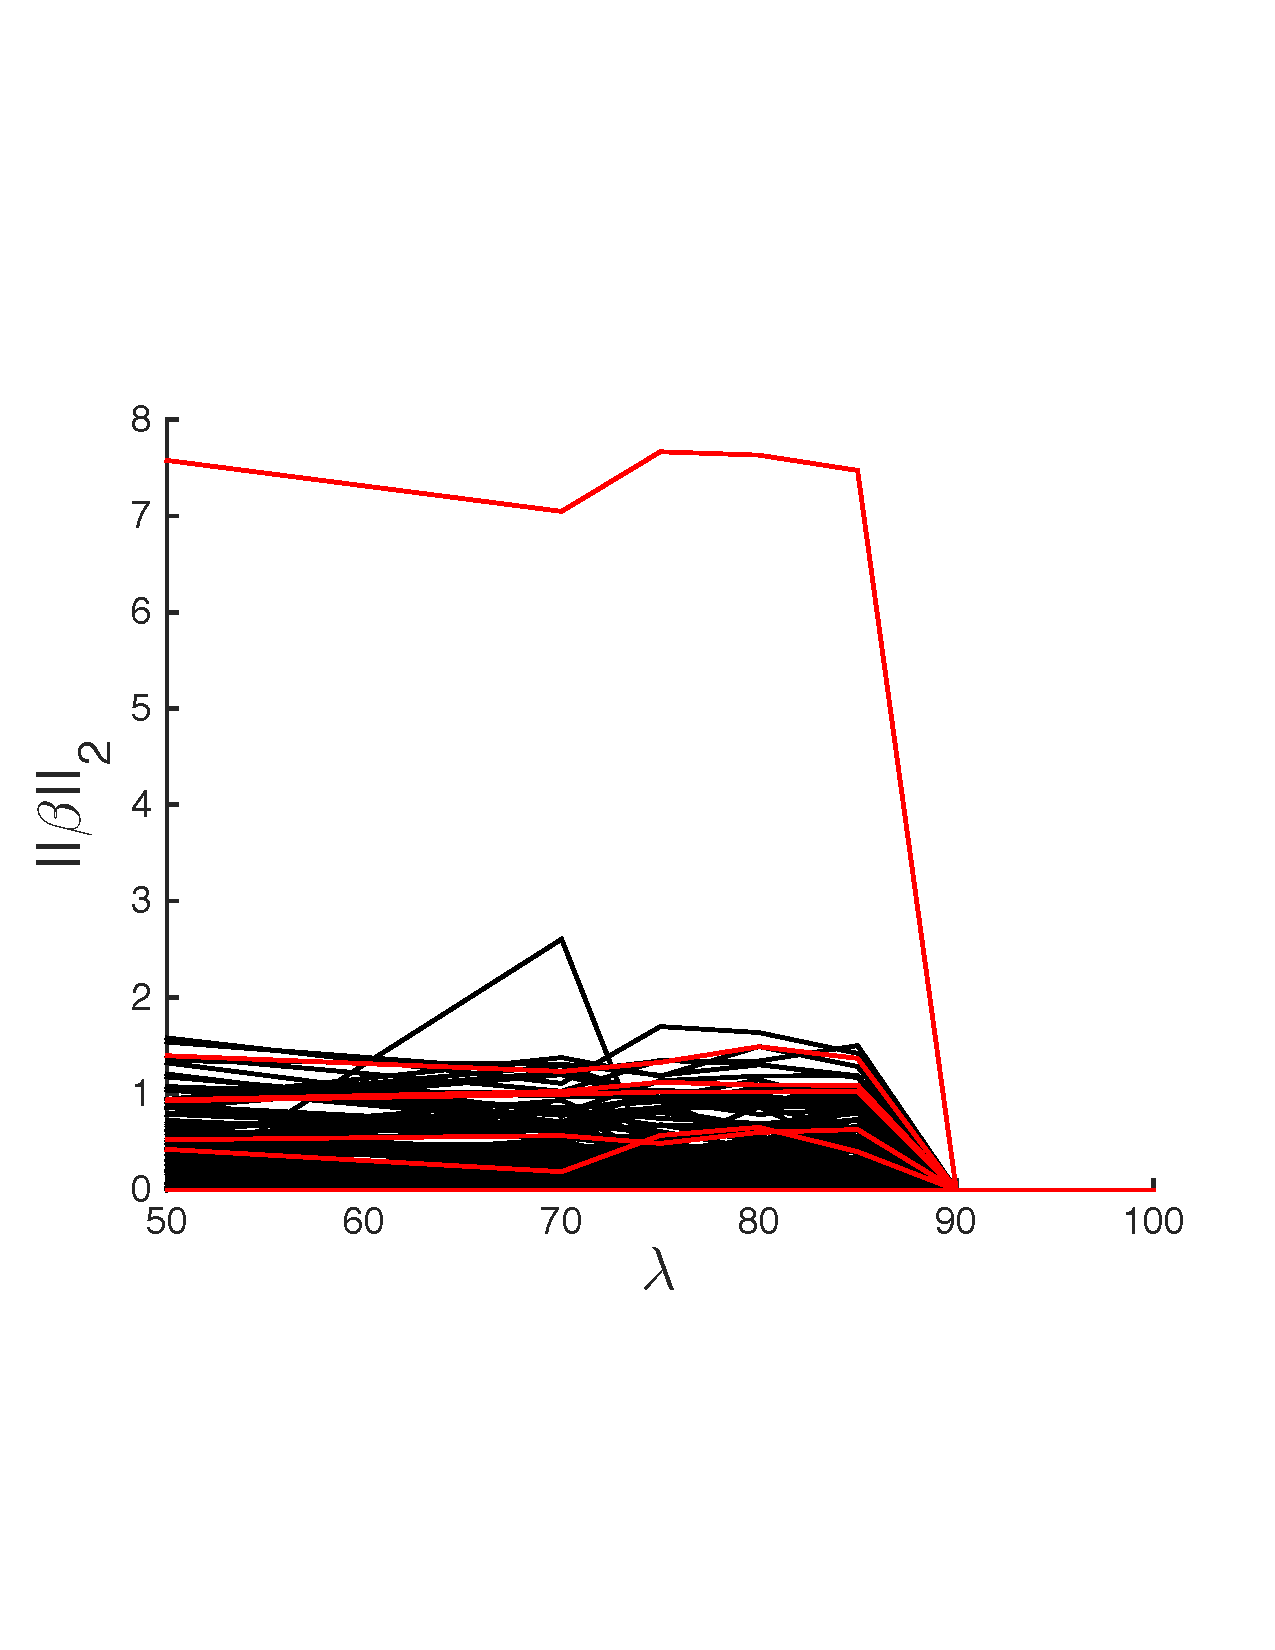
\includegraphics[width=3.4in]{figs/solnpath200.pdf}
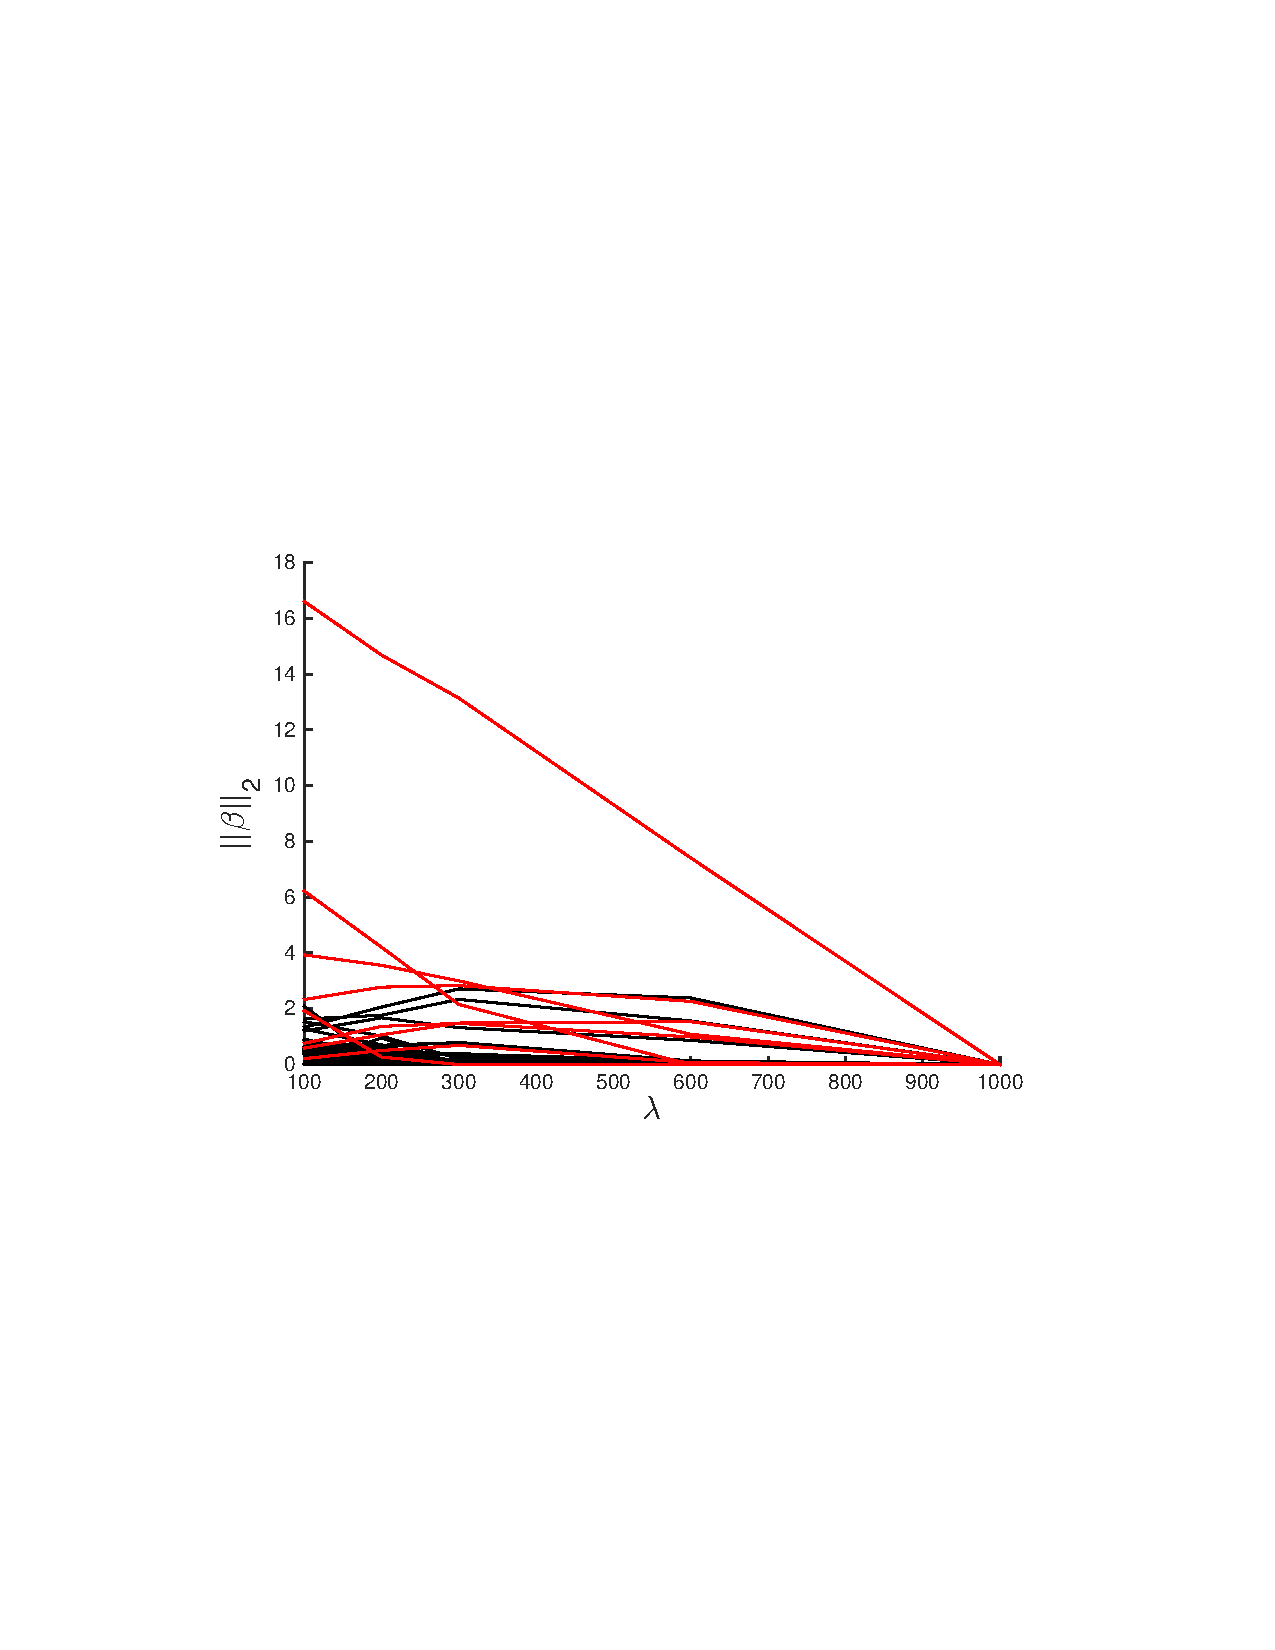
\includegraphics[width=3.2in]{figs/solnpath600.pdf}
\vspace{\imcaptionspace}
\caption[]{\small Solution path with $n=200$ samples (above) and
$n=600$ (below). The $x$-axis shows the regularization parameter,
while the $y$-axis plots the $\ell_2$-norm of all $\beta_j$. The true nonzero functions are depicted in red.}
\vspace{\imtextspace}
\label{fig:n200}
\end{figure}

